
\documentclass[a4paper]{article}
\usepackage[margin=1in]{geometry}
\usepackage[english]{babel}
\usepackage[utf8]{inputenc}
\usepackage{amsmath,amsthm,amssymb}
\usepackage{graphicx}
\usepackage{epstopdf}
\usepackage{pdfpages}
\usepackage{float, algorithmic, algorithm2e, program}
\usepackage{tabularx}
\usepackage{longtable}
\newtheorem{theorem}{Theorem}
\newtheorem{definition}{Definition}[section]

\title{Bathtub Qualitative Reasoning}
\author{Nicola De Cao, Luca Falorsi, Govert Verkes}
\date{\today}

\begin{document}
\maketitle

\section{Problem}
	
\begin{figure}[H]
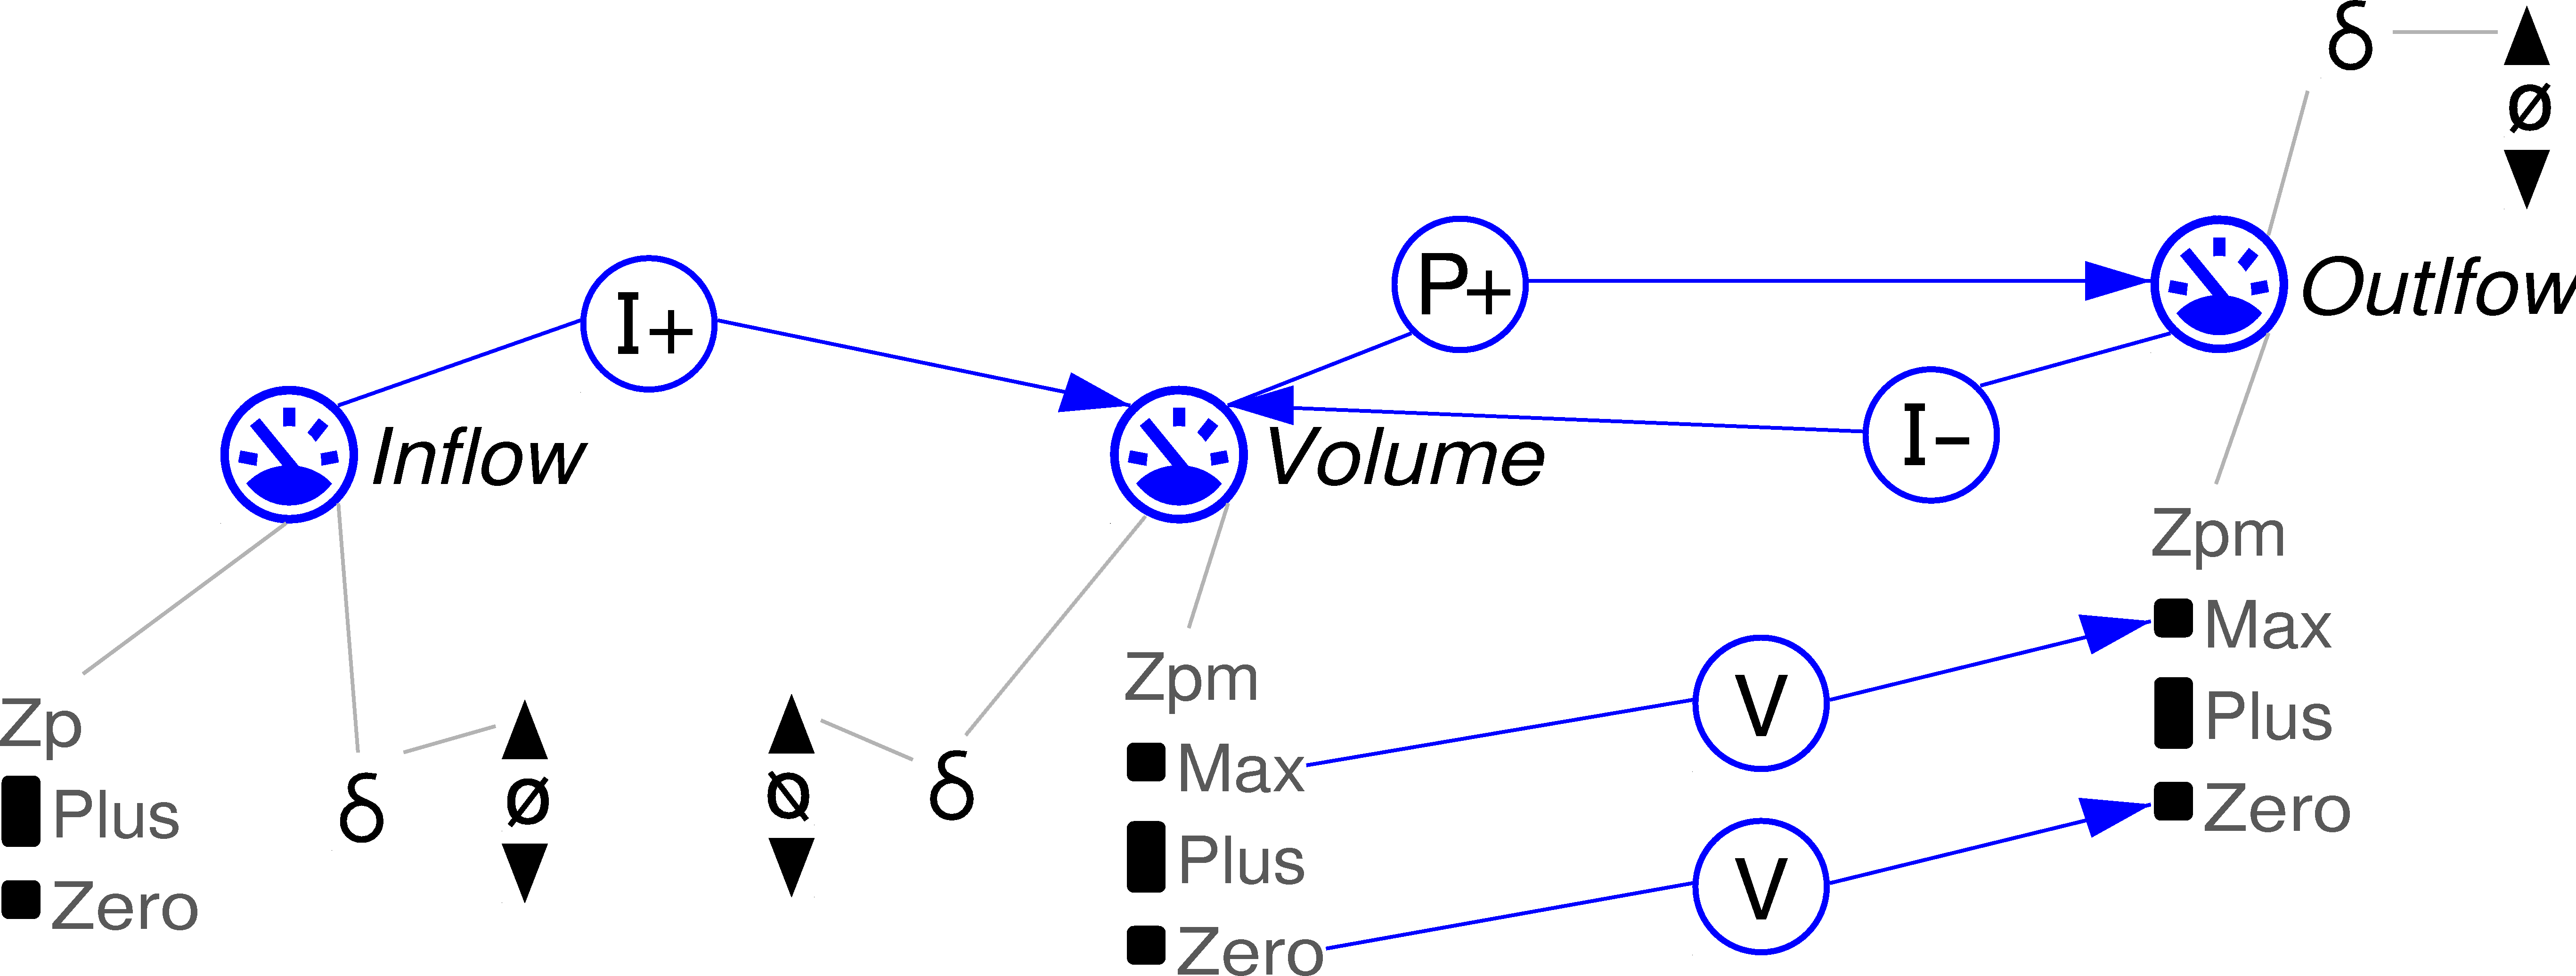
\includegraphics[]{problem.png}
\caption{Drawings of the causal model active for the system}
\end{figure}

\begin{algorithm}
\If{condition}{then-block}
\caption{Drawings of the causal model active for the system}
\end{algorithm}

\end{document}
 
